\documentclass[11pt, dvipdfmx]{beamer}
%\documentclass[8,9,10,11,12,14,17,20pt, dvips, handout]{beamer}
%%%%%%%%%%%  package  %%%%%%%%%%%
\usepackage{amssymb,amsmath,ascmac}
\usepackage{atbegshi}

\AtBeginShipoutFirst{\special{pdf:tounicode 90ms-RKSJ-UCS2}}
\usepackage{minijs}
\renewcommand{\kanjifamilydefault}{\gtdefault}
\usepackage{multirow}
\usepackage{bm}
%\usepackage[dvipdfmx]{graphicx}
%\usepackage{multimedia}

\usepackage{tikz}
\usepackage{xparse}
\usetikzlibrary{shapes,arrows}
%% define fancy arrow. \tikzfancyarrow[<option>]{<text>}. ex: \tikzfancyarrow[fill=red!5]{hoge}
  \tikzset{arrowstyle/.style n args={2}{inner ysep=0.1ex, inner xsep=0.5em, minimum height=2em, draw=#2, fill=black!20, font=\sffamily\bfseries, single arrow, single arrow head extend=0.4em, #1,}}
  \NewDocumentCommand{\tikzfancyarrow}{O{fill=black!20} O{none}  m}{
    \tikz[baseline=-0.5ex]\node [arrowstyle={#1}{#2}] {#3 \mathstrut};}

%微分関連のマクロ
%
\newcommand{\diff}{\mathrm d}
\newcommand{\difd}[2]{\dfrac{\diff #1}{\diff #2}}
\newcommand{\difp}[2]{\dfrac{\partial #1}{\partial #2}}
\newcommand{\difdd}[2]{\dfrac{\diff^2 #1}{\diff #2^2}}
\newcommand{\difpp}[2]{\dfrac{\partial^2 #1}{\partial #2^2}}

%%%%%%%%%%%  theme  %%%%%%%%%%%

%%%%%
% Simple
%%%%%
%\usetheme{default}
%\usetheme{Pittsburgh}
%\usetheme{Rochester}
%\usetheme{Szeged}

%%%%%
% So So
%%%%%
%\usetheme{Singapore}
%\usetheme{CambridgeUS}
\usetheme{Copenhagen}
%\usetheme{Luebeck}
%\usetheme{Malmoe}
%\usetheme{Warsaw}

%%%%%
% No Heasder
%%%%%
%\usetheme{Madrid}
%\usetheme{Boadilla}

%%%%%
% No Footer
%%%%%
%\usetheme{Darmstadt}
%\usetheme{JuanLesPins}
%\usetheme{Montpellier}

%%%%%
% Color
%%%%%
%\usetheme{AnnArbor}

%%%%%
% Too much
%%%%%
%\usetheme{Berlin}
%\usetheme{Ilmenau}

%%%%%
% Right hand Side
%%%%%
%\usetheme{Goettingen}
%\usetheme{Marburg}

%%%%%
% Left hand Side
%%%%%
%\usetheme{PaloAlto}


%%%%%%%%%%%  inner theme  %%%%%%%%%%%
\useinnertheme{default}
%\useinnertheme{circles}
%\useinnertheme{inmargin}
%\useinnertheme{rectangles}
%\useinnertheme{rounded}


%%%%%%%%%%%  outer theme  %%%%%%%%%%%
\useoutertheme{default}
%\useoutertheme{miniframes}
%\useoutertheme{infolines}
%\useoutertheme{miniframes}
%\useoutertheme{smoothbars}
%\useoutertheme{sidebars}
%\useoutertheme{split}
%\useoutertheme{shadow}
%\useoutertheme{tree}
%\useoutertheme{smoothtree}


%%%%%%%%%%%  color theme  %%%%%%%%%%%
%\usecolortheme{structure}
%\usecolortheme{sidebartab}
%\usecolortheme{albatross}
%\usecolortheme{beetle}
%\usecolortheme{dove}
%\usecolortheme{crane}
%\usecolortheme{fly}
%\usecolortheme{seagull}
%\usecolortheme{wolverine}
%\usecolortheme{beaver}
%\usecolortheme{lily}
%\usecolortheme{orchid}
%\usecolortheme{rose}
%\usecolortheme{whale}
%\usecolortheme{seahorse}
%\usecolortheme{dolphin}


%%%%%%%%%%%  font theme  %%%%%%%%%%%
\usefonttheme{professionalfonts}
%\usefonttheme{default}
%\usefonttheme{serif}
%\usefonttheme{structurebold}
%\usefonttheme{structureserif}
%\usefonttheme{structuresmallcapsserif}


%%%%%%%%%%%  degree of transparency  %%%%%%%%%%%
%\setbeamercovered{transparent=30}

%\setbeamercolor{item}{fg=red}
\setbeamertemplate{items}[default]

%%%%%%%%%%%  numbering  %%%%%%%%%%%
%\setbeamertemplate{numbered}

\setbeamertemplate{navigation symbols}{}

\title
[MD シミュレーションによるネットワークポリマーのゴム弾性]
{MD シミュレーションによる\\ネットワークポリマーのゴム弾性}
\author[東亞合成 佐々木、大村]{佐々木裕}
\institute[東亞合成]{東亞合成}
\date{March 20, 2018}

\begin{document}

%%%%%
% 1 P
%%%%%
\begin{frame}\frametitle{}
	\titlepage
\end{frame}



%%%%%%%%%%%%%%%%%%%%%
\section{はじめに}
%%%%%%%%%%%%%%%%
\begin{frame}
\LARGE{はじめに}
\end{frame}
%%%%%%%%%%%%%%%%


\subsection{高分子材料と耐久性}

%%%%%%%%%%%%%%%%%%%%%%%%%%%%%%%%%%%%%%
\begin{frame}
\frametitle{高分子材料への期待}

地球温暖化対策の CO$_2$ 削減への一つの主要なアイテムとして、\\
{\Large
{\color{red}「自動車を中心とした運送機器の抜本的な軽量化」}
}\\
が提唱されている。
\begin{block}{高分子材料への期待}
	\begin{itemize}
	\item
	現行の鉄鋼主体$ \Rightarrow$ 高分子材料を含むマルチマテリアル化
	
	\item
	高分子材料によるマルチマテリアル化のポイント
		\begin{itemize}
		\item
		高い比強度の有効利用
		\item
		特徴を生かした適材適所 $\Leftrightarrow$ 適切な接合方法の選択
			\begin{itemize}
			\item
			{\color{red} 「接着接合」への高分子の利用}
			\item
			{\color{red} 「柔らかさを生かした弾性接着接合」への期待}
			\end{itemize}
		\item
		{\color{blue}耐久性が不明確(特に疲労破壊に対して)}
		\end{itemize}
	\end{itemize}
\end{block}
\end{frame}


%%%%%%%%%%%%%%%%%%%%%%%%%%%%
%\subsubsection{破壊工学の考え方}
%%%%%%%%%%%%%%%%%%%%%%%%%%%%%%
\begin{frame}
\frametitle{破壊工学の考え方}
\begin{exampleblock}{破壊工学の考え方}

\begin{itemize}
\item
系中にクラックが存在することを前提に材料の耐久性を評価
\item
\alert{「クラック近傍での応力集中を如何に抑制するか」}がポイント
\end{itemize}
\end{exampleblock}

\begin{columns}[totalwidth=1\textwidth]
\column{.5\textwidth}
\begin{alertblock}{破壊工学の観点から(微視的)}
	\begin{itemize}
		\item
		クラック先端での応力集中\\ \alert{応力拡大係数 $K_I$ で評価}
		\footnotesize
		\begin{align*}
		K_{I} = \sigma \sqrt{\pi c}
		\end{align*}
		\normalsize
		\item 
		クラック進展の抑制 \\
		$\Rightarrow$ 先端での\alert{局所降伏}\\
		降伏応力 $\sigma_Y$ に反比例
		\footnotesize
		\begin{align*}
		d \propto \left( \dfrac{K_I}{\sigma_Y} \right)^2
		\end{align*}
		\normalsize
	\end{itemize}
\end{alertblock}
\column{.5\textwidth}
	\centering
	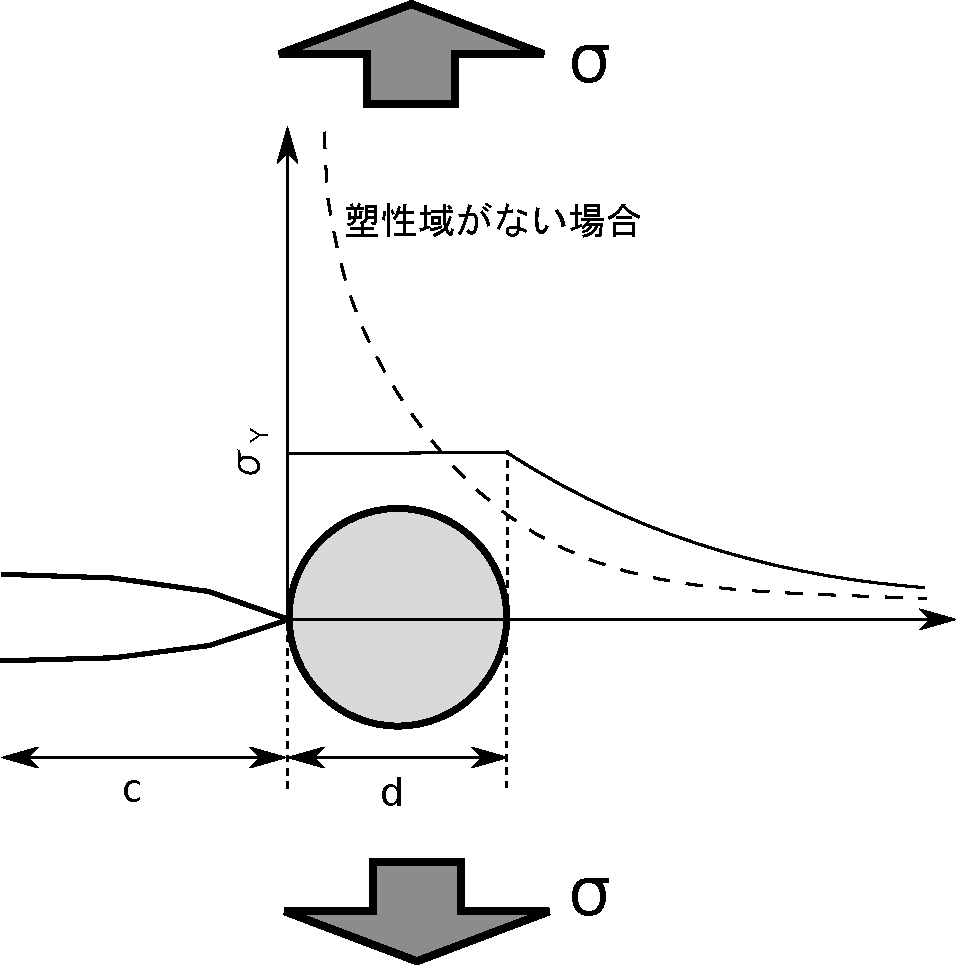
\includegraphics[width=45mm]{./fig/Crack_Yield.pdf}
\end{columns}

\end{frame}

\subsection{ゴムの力学特性と破壊耐性}


%%%%%%%%%%%%%%%%%
\begin{frame}
%[shrink squeeze]
\frametitle{ゴムの力学特性}

\begin{block}{ゴム材料の弾性}
	\begin{itemize}
	\item ゴム弾性はエントロピー由来であり{\color{red}本質的に可逆}。
	\begin{itemize}
		\item 適度な変形量では{\color{red} ミクロな破壊は考えにくい。}
	\end{itemize}
	\item 
	ゴムの複雑さ
	\begin{itemize}
		\item
		実在鎖としての、{\color{red}「伸びきり効果。」}
		\item ネオフッキアンモデル:
		線形バネの三次元繋がりで{\color{blue}非線形応答}。
		\item {\color{red} 降伏は無い。}
	\end{itemize}
	\end{itemize}
\end{block}

\begin{columns}[totalwidth=1\textwidth]
\column{.4\textwidth}
代表的なゴムのモデルの\\理論的 S-S カーブ
\begin{itemize}
\item
``Affine NW Model''
\item
伸び切り鎖モデル
\end{itemize}
\column{.6\textwidth}
\centering
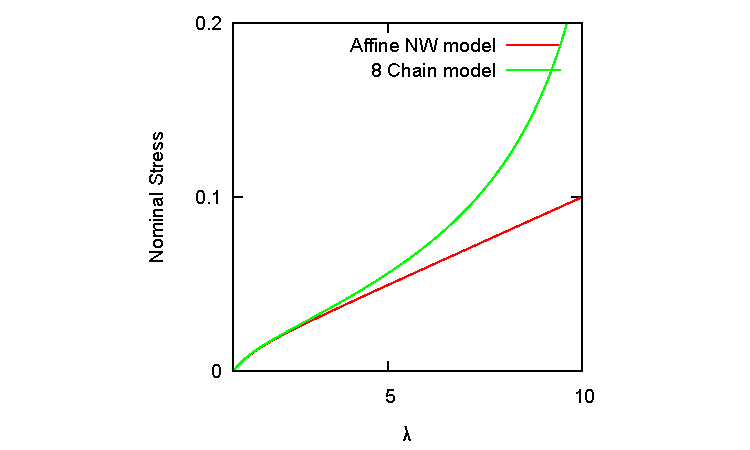
\includegraphics[width=60mm]{./fig/4_Chain.pdf}
\end{columns}

\end{frame}


%%%%%%%%%%%%%%%%%
\begin{frame}
\frametitle{ゴムの強靭性}


\begin{columns}[totalwidth=1\textwidth]
\column{.6\textwidth}
\begin{exampleblock}{Andrews 理論}
クラック先端の応力の等高線表示
	\begin{itemize}
	\item
	クラック成長時の応力場の考察より、
		\begin{itemize}
		\item
		{\color{red} Loading 場とUnloading 場の差}が重要。
		\item
		この差は\alert{ヒステリシスに由来}
		\end{itemize}	
	\item
	\alert{ひずみエネルギー開放率が低減} \\$\Rightarrow$ 強靭さの起源。
	\end{itemize}
\end{exampleblock}

{Andrews, E. H. and Fukahori, Y., Journal of Materials Science, 12, 1307 (1977)}

\column{.4\textwidth}
\centering
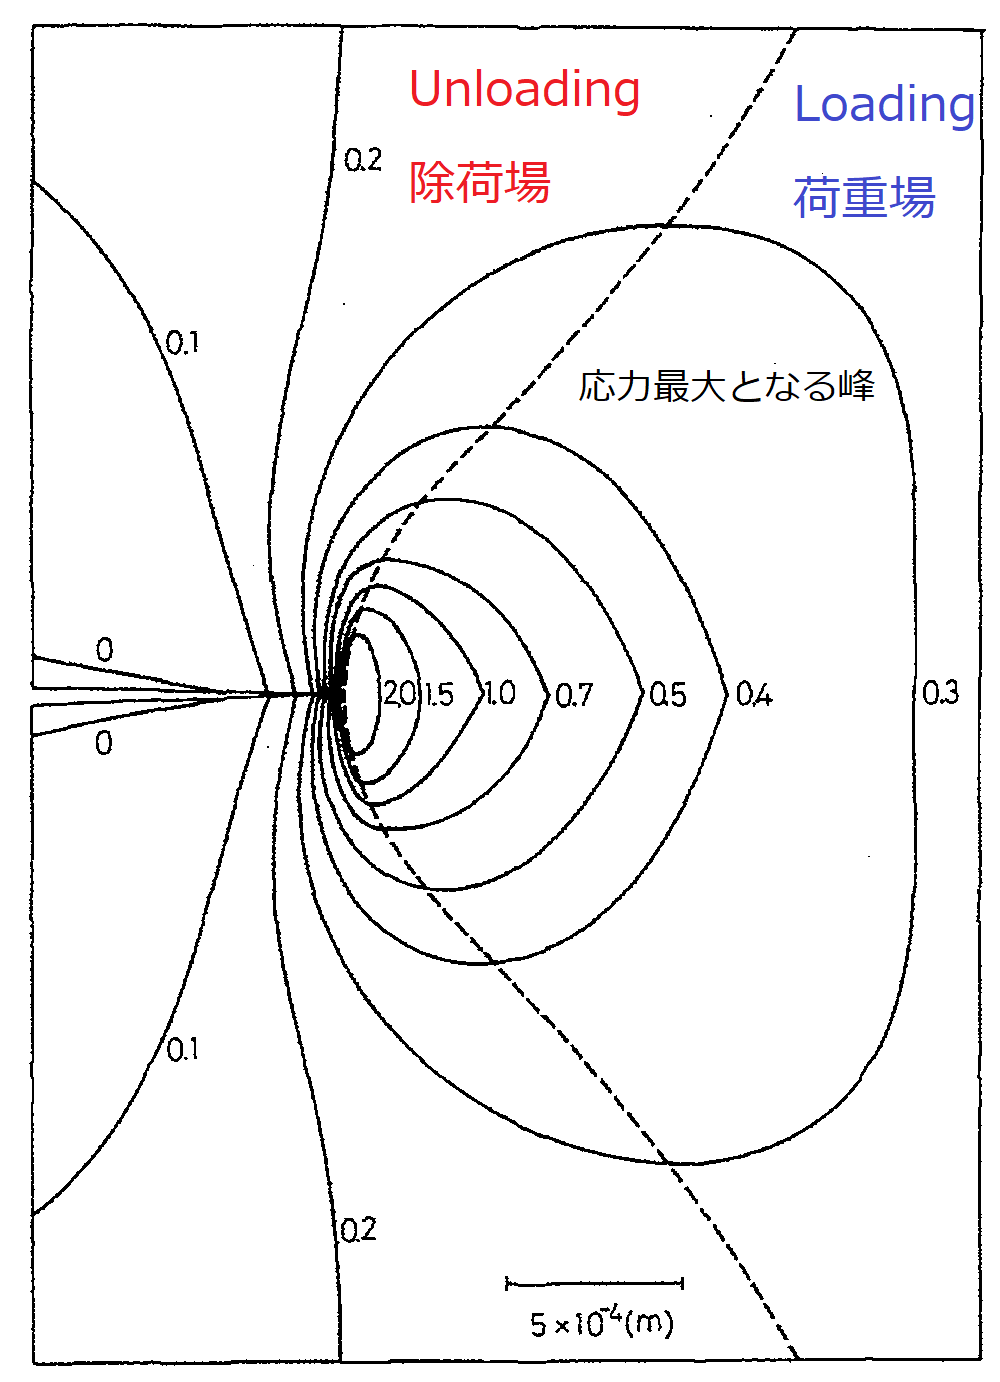
\includegraphics[width=40mm]{./fig/crack.png}
\end{columns}
\end{frame}


%%%%%%%%%%%%%%%%%
\begin{frame}
\frametitle{Mullins 効果}

\begin{columns}[totalwidth=1\textwidth]
\column{.45\textwidth}
Mullins 効果
	\begin{itemize}
		\item 歪み起因のヒステリシス
		\item (任意の緩和時間での)\\ \alert{内部構造の変化}
		\item 緩和時間と測定時間に\\応じて、\\{\color{red} 可逆} or 不可逆
	\end{itemize}
\column{.55\textwidth}
 \centering
	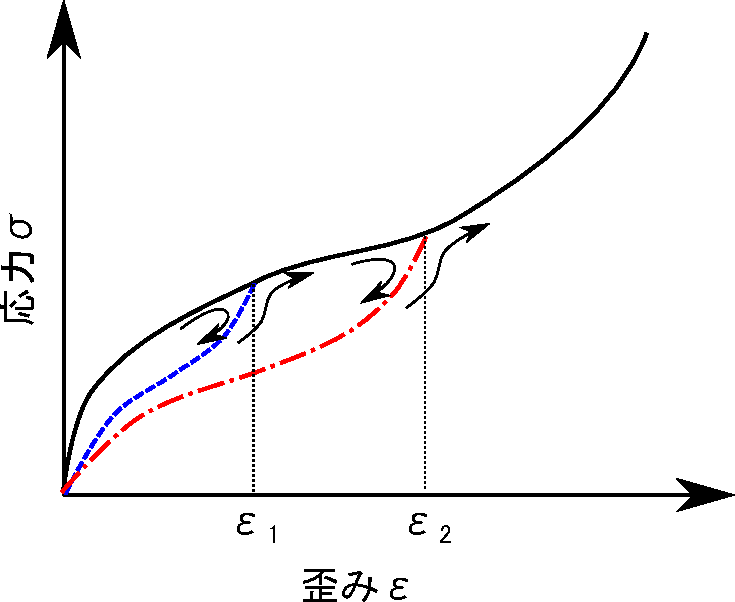
\includegraphics[width=65mm]{./fig/Mullins_Efct.pdf}
\end{columns}

\end{frame}


%%%%%%%%%%%%%%%%%%%%%%%%%%%%
\begin{frame}
\frametitle{ヒステリシス特性(実験系の例)}

\begin{columns}[totalwidth=1\textwidth]
\column{.4\textwidth}

{\Large 実験系の例}

\small
\begin{block}{実験条件}
\begin{itemize}
\item
チャック間距離:20mm
\item
伸長速度:10mm/min.
\end{itemize}
\end{block}

\begin{alertblock}{除荷時の挙動}
\begin{itemize}
\item
早い構造緩和
\item
ファントムモデルへの漸近
\end{itemize}
\end{alertblock}
\column{.01\textwidth}
\column{.58\textwidth}
\centering
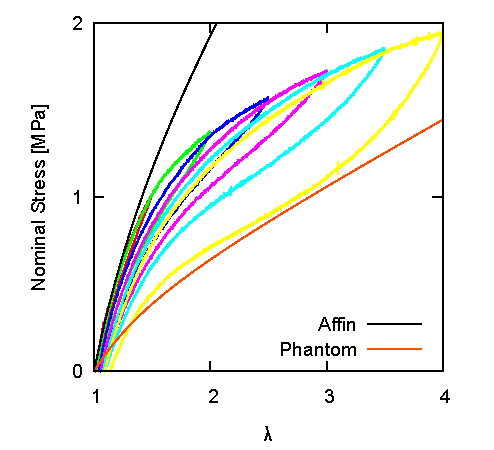
\includegraphics[width=70mm]{./fig/Hysteresis_10mm.pdf}

\end{columns}

\end{frame}



%%%%%%%%%%%%%%%%%%%%%%%%%%%%%%%
\begin{frame}
\frametitle{伸び切り鎖の効果(実験系の例)}

\begin{columns}[totalwidth=1\textwidth]
\column{.45\textwidth}

{\Large 実験系の例}

\small
$N_K\simeq50$
	\begin{itemize}
	\item
	$C_{\infty} \simeq 6$
	\item
	Mn$\simeq$6600
	\end{itemize}
%\item
%$E=2(C_1+C_2)/3$\\
%as Phantom NW model
%\end{itemize}

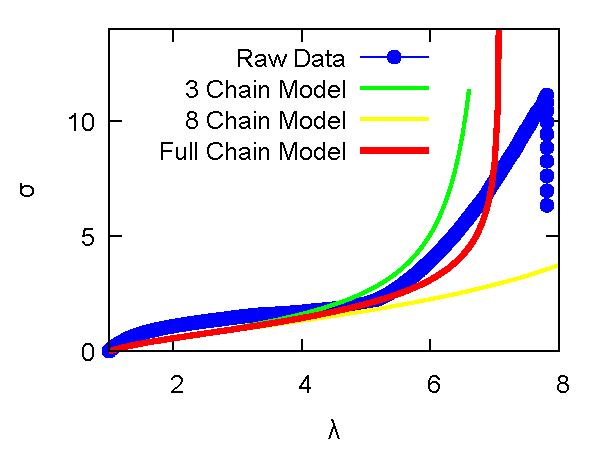
\includegraphics[width=50mm]{./fig/SS_6_Stretch.pdf}

\column{.04\textwidth}
\column{.5\textwidth}
\footnotesize
3-Chain model
\tiny
\begin{align*}
\sigma_{3ch}
	&= E\dfrac{\sqrt{N} }{3 } 
		\left[ 
			\mathcal{L}^{-1} \left(\dfrac{\lambda}{ \sqrt{N} } \right) 
			- \lambda^{-\dfrac{3}{2}} \mathcal{L}^{-1} \left( \dfrac{1}{ \sqrt{\lambda N} } \right)
		\right]
\end{align*}

\footnotesize
8-Chain model
\tiny
\begin{align*}
\sigma_{8ch}
	&= \dfrac{\nu k_B T }{3}\sqrt{N}
			\mathcal{L}^{-1} \left(\dfrac{\lambda_{chain}}{ \sqrt{N} } \right)
			\dfrac{\lambda-\dfrac{1}{\lambda^2}}{\lambda_{chain}} 
\end{align*}

\footnotesize
Full-Chain Model
\tiny
\begin{align*}
&\sigma_{Full} = E \dfrac{\sqrt{N}}{4\pi} \\
&\times \int_0^{\pi} \int_0^{2\pi} \mathcal{L}^{-1} \left( \dfrac{\lambda}{\sqrt{N}} \right) \dfrac{\lambda_i^2 m_i^2}{\lambda} \sin \theta \mathrm{d} \theta \mathrm{d} \phi \\
&m_0 = \sin \theta \cos \theta,\; m_1 = \sin \theta \sin \phi,\\
&m_2 = \cos \theta,\;\lambda^2 = \sum_{i=0}^2 \lambda_i^2m_i^2
\end{align*}
\normalsize
\end{columns}
\end{frame}


%%%%%%%%%%%%%
\begin{frame}
\frametitle{ターゲット}

破壊耐性に優れた軽量材料の候補として「ゴム材料」を捉えれば、


\begin{block}{設計のポイント}
\begin{itemize}
\item
可逆性の有効利用
	\begin{itemize}
	\item
	可逆性の高いヒステリシスの設計
	\end{itemize}
\item
弾性限界の設計
	\begin{itemize}
	\item
	伸びきり効果の明確化
	\end{itemize}
\end{itemize}
\end{block}

\begin{alertblock}{シミュレーションでやりたいこと}
\begin{itemize}
\item
上記二つのポイントの指針を得たい。
\item
できるだけ単純化したモデルから始めたい。
\end{itemize}
\centering
\Large
\color{red}「オッカムの剃刀」
\end{alertblock}

\end{frame}


%%%%%%%%%%%%%%%%%%%%%%
\subsection{本発表の内容}
%%%%%%%%%%%%%%%%%%%%%%%%%%
\begin{frame}
\frametitle{本発表の内容}

\begin{exampleblock}{本研究の目標とアプローチ}
\begin{itemize}
\item
目標\\
破壊耐性に優れた軽量材料の創成とその設計指針の明確化
\item
アプローチ
	\begin{itemize}
	\item
	可逆性に優れた材料としてゴム材料を選択。
	\item
	構造明確なネットワークの構築のために超分子ネットワーク。
	\item
	既知のモデルとの整合性を確認。
	\item
	\color{red}シミュレーションの併用でマルチスケールモデルを構築\color{black}
	\end{itemize}
\end{itemize}
\end{exampleblock}


\begin{block}{本発表の内容}
本発表では、単純化したネットワークモデルをMDシミュレーションにより検討した結果について報告を行う。
\end{block}
\end{frame}

%%%%%%%%%%%%%%%%%%%%%%%%%%%%%%
\section{MD シミュレーション結果}
%%%%%%%%%%%%%%%%%%%%%%%%%%%%%%

%%%%%%%%%%%%%%%%%%%%%
\begin{frame}
\Large{KG ポリマーによるネットワークの\\MDシミュレーション}
\end{frame}
%%%%%%%%%%%%%%%%%%%%%%%
\subsection{KG ポリマーによるネットワークのMDシミュレーション}
%%%%%%%%%%%%%%%%%%%
\begin{frame}
\frametitle{検討の対象}

\begin{block}{KG ポリマーによるネットワーク}
	\begin{itemize}
	\item ストランドにKG ポリマー
		\begin{itemize}
		\item ビーズ間には LJ ポテンシャル
		\item ビーズを繋ぐボンドに FENE-LJ ポテンシャル
		\end{itemize}
	\item 特徴
		\begin{itemize}
		\item 「排除体積効果」および「絡み合い」
		\item 伸びきり鎖も評価できる。
		\end{itemize}
	\item ネットワーク構造
		\begin{itemize}
		\item ダイヤモンド構造ベースの 4-Chain モデル
	%	\item 単純格子ベースの 6-Chain モデル
	%	\item 体心立方ベースの 8-Chain モデル
		\end{itemize}
	\end{itemize}
\end{block}

\begin{alertblock}{先行研究}
R. Everaers, New J. Phys. 1999, 1, 12.
\end{alertblock}

\end{frame}


%%%%%%%%%%%%%%%%%%%%%%%%%%%%%%%
\begin{frame}
\frametitle{IPNによる密度の調整}

\begin{alertblock}{IPNによる密度の調整}
ストランド長を理想状態での末端間距離としてシステムの密度を設定($\rho = 0.85$)するため、ネットワークを多重化(IPN)した。
\end{alertblock}

\begin{columns}[totalwidth=1\textwidth]
\column{.48\textwidth}

\footnotesize
KG 鎖の末端間距離は、
\vspace{-3mm}
\begin{align*}
r \simeq \sqrt{1.7 \times \text{Bonds}}\times b \quad(b=0.97)
\end{align*}

\vspace{-3mm}
単位セルの長さは、
\vspace{-3mm}
\footnotesize
\begin{align*}
\color{red}
a= \dfrac{4 r}{\sqrt{3}}
\end{align*}

\column{.48\textwidth}

\footnotesize
単位セル中のセグメント数は、
\vspace{-3mm}
\begin{align*}
N_{UC}&= 8+16N
\end{align*}

\vspace{-3mm}
システムの密度は、
\vspace{-3mm}
\begin{align*}
\rho&=\dfrac{8+16N}{a^3}
\end{align*}
\end{columns}

\vspace{-3mm}
\begin{table}[htb]
 \centering
	\scriptsize
 \begin{tabular} {|c|c|c|c|c|c|c|c|} \hline
Segments	& Bonds	& Strand Length	& Cell Size	& \multicolumn{4}{|c|}{$\rho$}			\\ \cline{5-8}
b/w J.P. 	& b/w J.P.	& $r$		& $a$				& $n=1$	& $n=2$	& $\cdots$	& $n=9$	\\ \hline \hline
%1			&	2	&	1.372		& 3.168		& 0.755	& 1.510	& 2.265	& 3.019	\\ \hline
%2			&	3	&	1.680		& 3.880		& 0.685	& 1.370	& 2.054	& 2.739 \\ \hline
%$\vdots$	& \multicolumn{7}{|c|}{} \\ \hline
%9			&	10	&	3.067		& 7.084		& 0.428	& {\color{red}0.855}	& 1.283	& 1.710	\\ \hline
%$\vdots$	& \multicolumn{7}{|c|}{} \\ \hline
%23			&	24	&	4.752		&	10.974	& 0.284	& 0.569	& {\color{red}0.853}	& 1.138	\\ \hline
%$\vdots$	& \multicolumn{7}{|c|}{} \\ \hline
44			&	45	&	8.484		&	19.593	& 0.0947	& 0.189	& $\cdots$	& {\color{red}0.852} 		\\ \hline
\end{tabular}
\end{table}
\end{frame}

%%%%%%%%%%%%%%%%%%%%%%%%%%%%%%%%%
\begin{frame}
\frametitle{MD シミュレーション}

OCTA 上の Cognac により、MD シミュレーションを実施。

\begin{columns}[T, totalwidth=1\linewidth]
\column{.5\linewidth}
\begin{block}{シミュレーション条件}
	\begin{itemize}
	\item
	KG モデル
	\item
	構造:ダイヤモンド構造
	\begin{itemize}
		\item
		ストランド長:44
		\item
		架橋点/ ユニット:8
		\item
		ストランド/ ユニット:16
		\item
		ユニット数:$2 \times 2 \times 2$
		\item
		多重度:9
		\item
		密度 $\rho =0.85$
	\end{itemize}
	
	\item
	緩和条件:\\
	NPTで所定の密度 $\Rightarrow$ NVT
	\end{itemize} 
\end{block}
\column{.01\linewidth}
\column{.45\linewidth}
初期状態($\rho \simeq 0.2$)
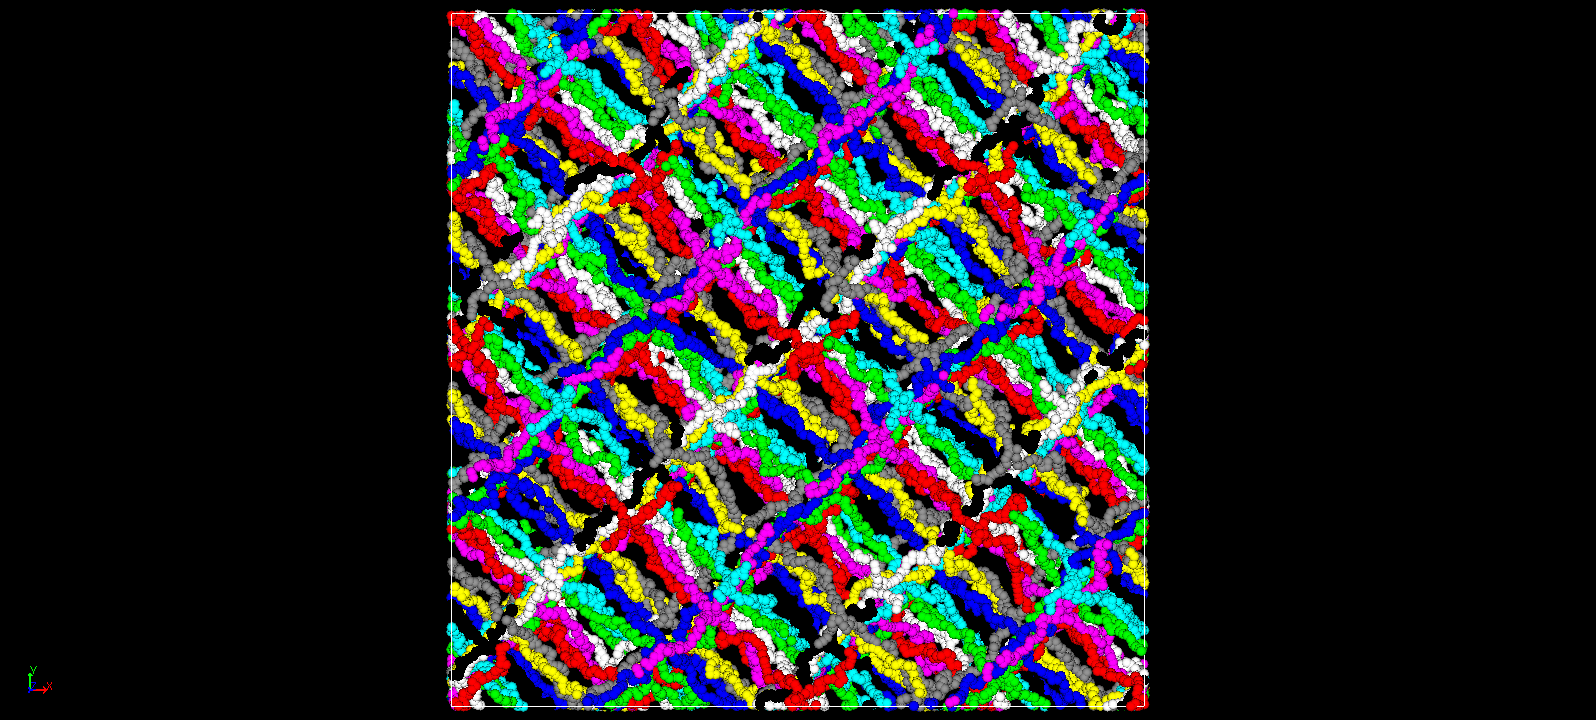
\includegraphics[width=\columnwidth]{./fig/Init.png}

\vspace{-3mm}
\begin{center}
$\Downarrow$ NPT
\end{center}
\vspace{-3mm}

初期緩和後($\rho =0.85$)
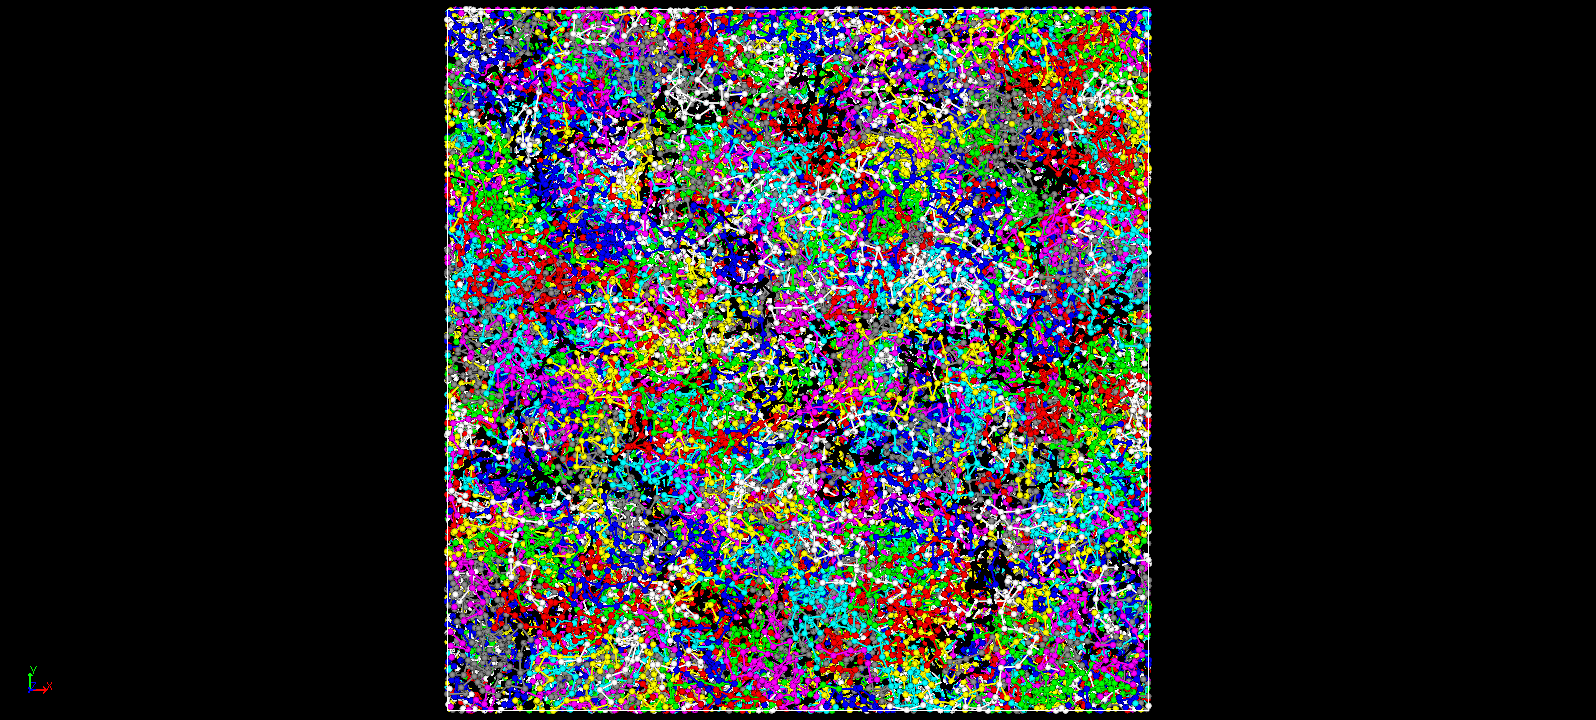
\includegraphics[width=\columnwidth]{./fig/after.png}
\end{columns}
\end{frame}



%%%%%%%%%%%%%%%%%%%%%%%%%%%%%
\subsection{シミュレーション結果}
%%%%%%%%%%%%%%%%%%%%%%%%%%%%%
\begin{frame}
\Large{シミュレーション結果\\静的構造}
\end{frame}
%%%%%%%%%%%%%%%%%%%%%%%%%%%%%%%%%%%%%%%%%%
\begin{frame}
\frametitle{平衡状態での末端間距離の分布 $P_{strand}(z)$ (N=44) }

\begin{columns}[totalwidth=1\textwidth]
\column{.5\textwidth}
\footnotesize
ダイヤモンド構造のネットワークで、ストランド末端間距離の $z$ 成分の分布関数 $P_{strand}(z)$ は、
\vspace{-3mm}
\tiny
%footnotesize
\begin{align*}
P_{strand}(z) 
&= \dfrac{1}{2}\dfrac{1}{\sqrt{2\pi}\Delta_1^z} \\
&\quad \times \left[ \exp\left(-\dfrac{(z-Z_1)^2}{2(\Delta^z_1)^2} \right) \right. \\
&\quad \quad \left. + \exp\left(-\dfrac{(z+Z_1)^2}{2(\Delta^x_1)^2} \right) \right]
\end{align*}
ただし、ボンド数 $M=45$ より、\\
$R_0^2=1.75*45*(0.97)^2$ = 74.1
$Z_1=\sqrt{\dfrac{R_0^2}{3}} =4.97$、
$\Delta^z_1=\sqrt{\dfrac{2}{f}}Z_1 = 3.51$

\column{.5\textwidth}
\centering
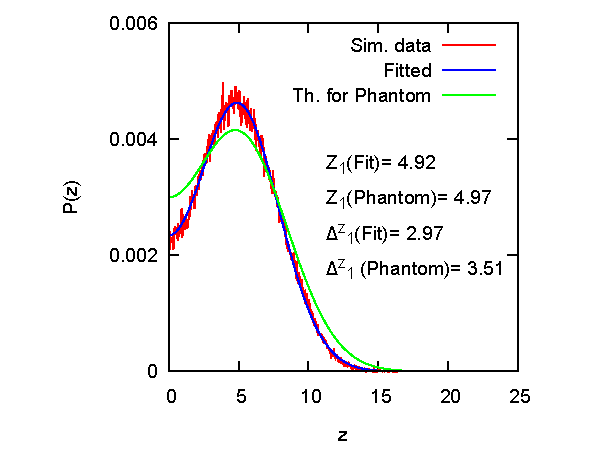
\includegraphics[width=70mm]{./fig/Rz.pdf}
\end{columns}

\scriptsize
\begin{block}{ファントム鎖との比較}
\begin{itemize}
\item
図中に示したように、ファントム鎖と比較して架橋点での揺らぎが抑制されていた。
\item
これは、KG 鎖ではストランド間でのすり抜けが抑制され、隣のストランドにより圧迫されているためと考えられる。
\end{itemize}

\end{block}
\end{frame}

%%%%%%%%%%%%%%
\begin{frame}
\frametitle{KG鎖のアングル}

\small
KG 鎖では、1,3 位のセグメント間に働く LJ ポテンシャル に起因した反発によりアングルが定まる。\\
このとき、アングルの平均値は以下のように見積もれる。


\begin{columns}[totalwidth=1\textwidth]
\column{.6\textwidth}
\tiny
\begin{align*}
&\langle \cos (\theta) \rangle 
= \dfrac{
\displaystyle \int_0^{\pi} \rm{d} \theta 
\sin(\theta) 
\color{red}
\cos(\theta)
\color{black} 
\exp \left(-\dfrac{U_{LJ}(r(\theta))}{k_B T}\right)
}
{\displaystyle \int_0^{\pi} \rm{d} \theta 
\sin(\theta) \exp \left(-\dfrac{U_{LJ}(r(\theta))}{k_B T}\right)}
\simeq 0.274 \notag \\
&\theta \simeq 74.1
\end{align*}

ただし、
\begin{align*}
r(\theta)&=2b \sin \left( \dfrac{\pi-\theta}{2} \right) \notag \\[12pt]
U_{LJ}(r) &= 
\begin{cases}
4 \epsilon\left[\left(\dfrac{\sigma}{r}\right)^{12} - \left(\dfrac{\sigma}{r}\right)^{6} + \dfrac{1}{4} \right] \;\;\; & r< 2^{1/6} \sigma \\[8pt]
0 \;\;\; & r \geq 2^{1/6} \sigma
\end{cases}
\end{align*}

\column{.4\textwidth}
\begin{center}
\small
アングルのヒストグラム
\end{center}

\vspace{-10mm}
\begin{figure}
\centering
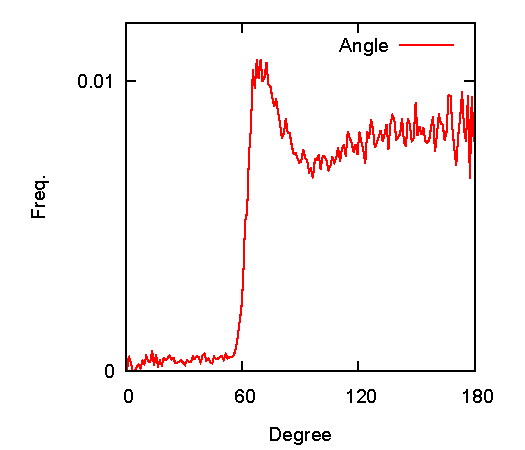
\includegraphics[width=50mm]{./fig/Angle_Init.pdf}
\end{figure}
\end{columns}

\end{frame}

%%%%%%%%%%%%%%%%%%%%%%%%%%%%%
\begin{frame}
\Large{シミュレーション結果\\一軸伸長}
\end{frame}
%%%%%%%%%%%%%%%%%%%%%%%%%%%%%%%%%%%%%%%%%%

%%%%%%%%%%%%%%%%%
\begin{frame}
\frametitle{一軸伸長}

\begin{columns}[totalwidth=1\textwidth]
\column{.46\textwidth}

\begin{block}{一軸伸長}
\begin{itemize}
\footnotesize
\item
伸長度小($\lambda \leq 3$)

伸長速度($\sigma/\tau$)の低下により、ネオフッキアン(NH)に漸近。

\item
$\lambda \geq 3$
	\begin{itemize}
	\footnotesize
	\item
	伸びきりによる応力上昇は再現
	\item
	``4-Chain model'' より早く応力増加。
	\end{itemize}
\end{itemize}
\end{block}

\footnotesize
4-Chain model
\tiny
\begin{align*}
\sigma_{8ch}
	&= \dfrac{\nu k_B T }{3}\sqrt{N}
			\mathcal{L}^{-1} \left(\dfrac{\lambda_{chain}}{ \sqrt{N} } \right)
			\dfrac{\lambda-\dfrac{1}{\lambda^2}}{\lambda_{chain}} 
\end{align*}

\column{.06\textwidth}
\column{.46\textwidth}
%\centering
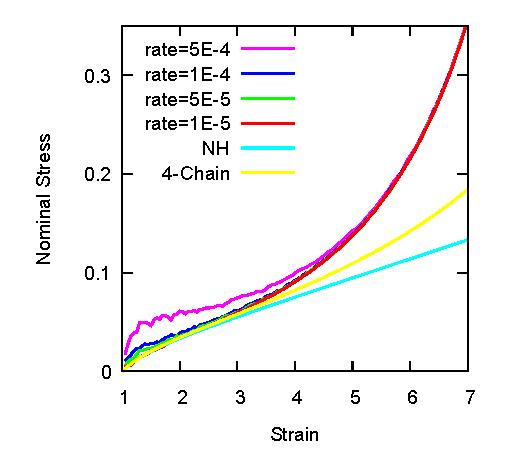
\includegraphics[width=60mm]{./fig/SS.pdf}

%\footnotesize
%4-Chain model
%\tiny
%\begin{align*}
%\sigma_{8ch}
%	&= \dfrac{\nu k_B T }{3}\sqrt{N}
%			\mathcal{L}^{-1} \left(\dfrac{\lambda_{chain}}{ \sqrt{N} } \right)
%			\dfrac{\lambda-\dfrac{1}{\lambda^2}}{\lambda_{chain}} 
%\end{align*}

\tiny
\begin{align*}
\sigma_{T} = \sigma_{zz} -\dfrac{1}{2}(\sigma_{xx}+\sigma{yy})
\end{align*}

\end{columns}

\end{frame}


%%%%%%%%%%%%%%%%%%%%%
\begin{frame}
%[shrink squeeze]
%[allowframebreaks]
\frametitle{伸長度小($\lambda \leq 3$)での挙動}

\small
\begin{alertblock}{ムーニー・リブリンプロット}
伸長速度 $\sigma/\tau = 1E^{-5}$ [$\sigma/\tau$] において、$C2=0$

ネオフッキアンモデルに合致することが確認できた。
\end{alertblock}

\begin{columns}[T, totalwidth=0.96\linewidth]
\column{.47\linewidth}

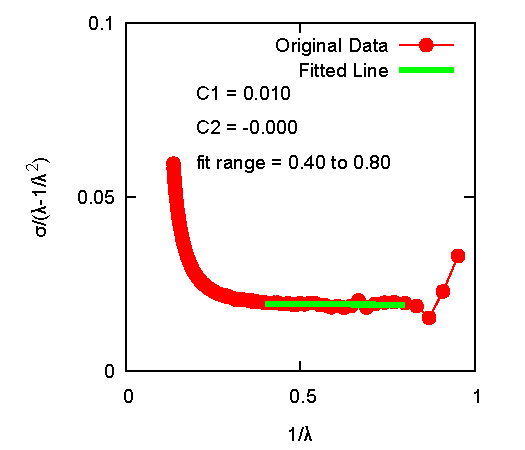
\includegraphics[width=\columnwidth]{./fig/MR_1e-5.pdf}
\column{.47\linewidth}

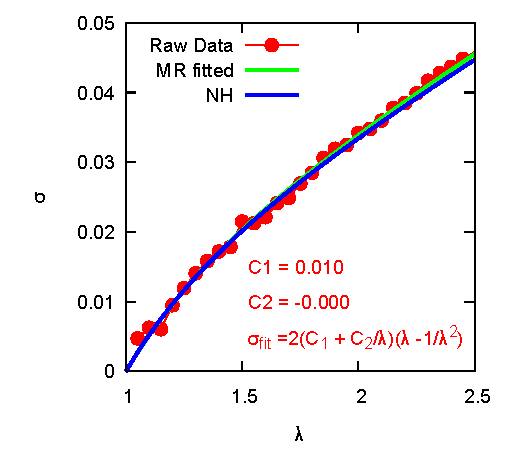
\includegraphics[width=\columnwidth]{./fig/SS_w_MR_1e-5.pdf}
\end{columns}
\end{frame}

%%%%%%%%%%%%%%%%%%%%%%%%%%%%%%%%%%
\begin{frame}
\frametitle{Edwards Vilgis model}

\begin{columns}[totalwidth=1\textwidth]
\column{.5\textwidth}

\tiny
絡み合いの効果を考慮したモデルとして、下式の Edwards Vilgis model が知られている。

$\eta$ は、絡み合いに起因したポリマー鎖の摩擦を表す因子

$\alpha$ は、伸び切り鎖の寄与を表す因子

\begin{align*}
f
	&= N_c D \left[ \dfrac{1-\alpha^2}{(1-\alpha^2 \phi)^2} - \dfrac{\alpha^2}{1-\alpha^2 \phi} \right]\notag \\
	&\quad + N_e \left[
			\dfrac{(1+\eta)(1-\alpha^2)\alpha^2D}{(1-\alpha^2 \phi)^2} \left\{ \dfrac{\lambda^2}{1+\eta \lambda^2}
				+\dfrac{2}{\lambda+\eta} \right\} \right. \notag \\
			&\quad\quad + \dfrac{1}{1-\alpha^2\phi} \left( \dfrac{\lambda}{(1+\eta \lambda^2)^2} -\dfrac{1}{(\lambda+\eta)^2} \right) \notag \\
			&\quad\quad \left. + \eta \dfrac{D \lambda}{(1+\eta\lambda^2)(\lambda + \eta)} -D\alpha^2\dfrac{1}{1-\alpha^2\phi}
		\right]
\end{align*}
なお、$\phi=\lambda^2-\dfrac{2}{\lambda}, D=\dfrac{\diff \phi}{\diff \lambda}$ である。

\column{.5\textwidth}
\begin{center}
伸長速度 $\sigma/\tau = 1E^{-5}$ [$\sigma/\tau$]
\end{center}
\vspace{-3mm}
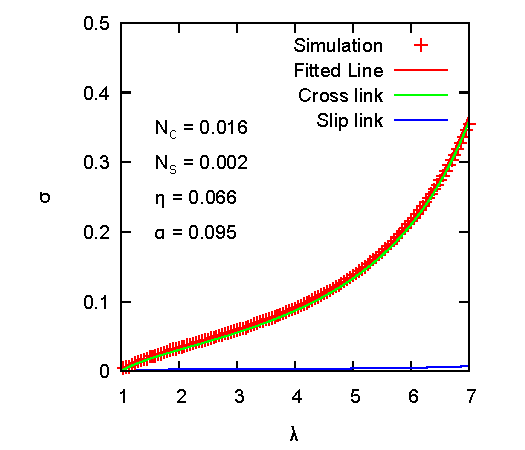
\includegraphics[width=\columnwidth]{./fig/E_V.pdf}
\end{columns}
\vspace{3mm}
\footnotesize
S. F. Edwards and Th. Vilgis, Polymer, 484, Vol 27 (1986)
\end{frame}

%%%%%%%%%%%%%%%%%%%%%%%%%%%%%%%%%%
\begin{frame}
\frametitle{Edwards Vilgis model}

\footnotesize
\begin{itemize}
\item
$\eta$ は、絡み合いに起因したポリマー鎖の摩擦を表す因子
\item
$\alpha$ は、伸び切り鎖の寄与を表す因子
\item
N$_c$, N$_s$ は、それぞれ、クロスリンク、スリップリンクの数を表す。
\end{itemize}

\vspace{-3mm}


\begin{columns}[totalwidth=1\textwidth]
\column{.5\textwidth}
\begin{center}
伸長速度 $\sigma/\tau = 5E^{-4}$ [$\sigma/\tau$]
\end{center}
\vspace{-3mm}
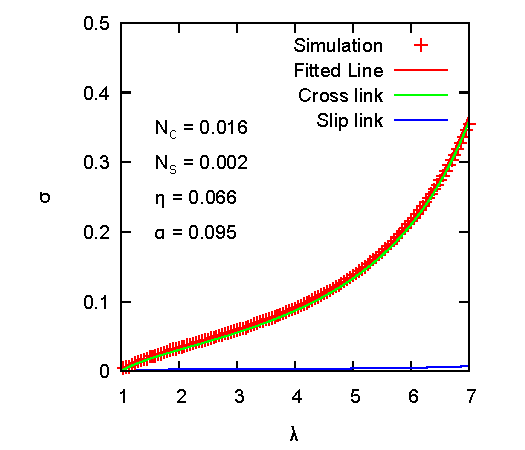
\includegraphics[width=\columnwidth]{./fig/E_V.pdf}

\column{.5\textwidth}
\begin{center}
伸長速度 $\sigma/\tau = 1E^{-5}$ [$\sigma/\tau$]
\end{center}
\vspace{-3mm}
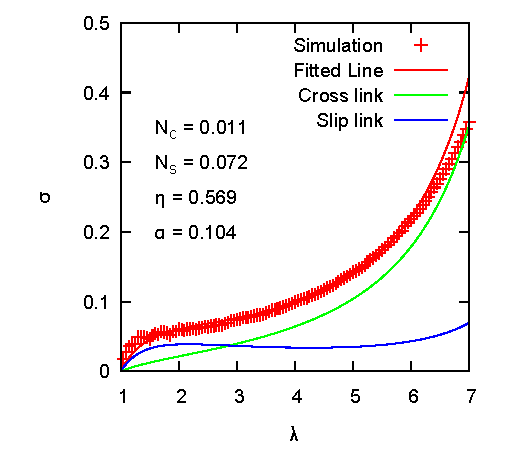
\includegraphics[width=\columnwidth]{./fig/E_V_5e-4.pdf}
\end{columns}
\end{frame}

%%%%%%%%%%%%%%%%%%%%%%%%%%%%%%%%%%%%%%%%%%%%%
\subsection{KG 鎖の特徴的なふるまいも考慮して}
%%%%%%%%%%%%%%%%%%%%%%%%%%%%%%%%%%%%%%%%%%%%%
%%%%%%%%%%%%%%%%%%%%%%%%%%%%%
\begin{frame}
\Large{シミュレーション結果\\KG 鎖の特徴的なふるまいも考慮して}
\end{frame}
%%%%%%%%%%%%%%%%%%%%%%%%%%%%%%%%%%%%%%%%%%

%%%%%%%%%%%%%
\begin{frame}
\frametitle{伸長速度の比較}

\begin{columns}[totalwidth=1\textwidth]
\column{.5\textwidth}
\begin{itemize}
\item
応力の由来により、ノンボンドとボンドに分割

\begin{itemize}
\item
伸長速度 $\sigma/\tau = 5E^{-4}$ [$\sigma/\tau$] では、ノンボンドの寄与が大きく増加
\item
セグメント間での相互作用が応力の増加に寄与。
\end{itemize}
\end{itemize}

\column{.5\textwidth}
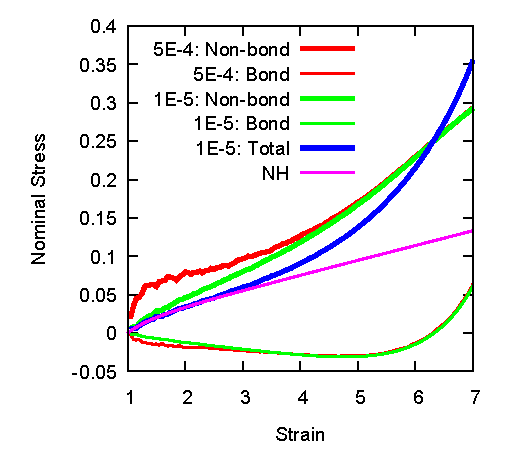
\includegraphics[width=\columnwidth]{./fig/SS_bond.pdf}
\end{columns}

\begin{block}{KG 鎖の振る舞い}
\begin{itemize}
\item
ボンド由来の応力項が負。
\item
ボンドポテンシャルの FENE-LJ の効果?
\end{itemize}
\end{block}

\end{frame}



%%%%%%%%%%%%%%
\begin{frame}
%[shrink squeeze]
%[allowframebreaks]
\frametitle{クーン長としての換算}

\begin{columns}[totalwidth=1\textwidth]
\column{.48\textwidth}
\small
\begin{alertblock}{KG 鎖を自由連結鎖に換算}
\begin{itemize}
\item
KG 鎖のアングルは、$\simeq74$
\item
このストランドのクーンセグメント数は $N_K\simeq16.6$ と換算
\item
伸びきり効果が発現する伸長比が低下。
\item
フィッティングでは、$N\simeq21$
\end{itemize}
\end{alertblock}

\footnotesize
4-Chain model
\tiny
\begin{align*}
\sigma_{8ch}
	&= \dfrac{\nu k_B T }{3}\sqrt{N}
			\mathcal{L}^{-1} \left(\dfrac{\lambda_{chain}}{ \sqrt{N} } \right)
			\dfrac{\lambda-\dfrac{1}{\lambda^2}}{\lambda_{chain}} 
\end{align*}

\column{.5\textwidth}
\centering
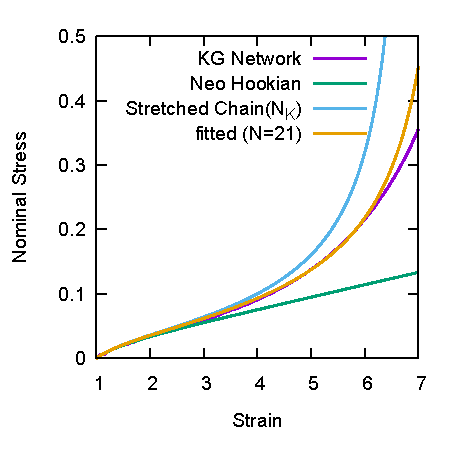
\includegraphics[width=\columnwidth]{./fig/SS_Kuhn.pdf}

\end{columns}
\end{frame}

%%%%%%%%%%%%%%
\begin{frame}
%[shrink squeeze]
%[allowframebreaks]
\frametitle{伸長時のアングル}

\begin{columns}[totalwidth=1\textwidth]
\column{.5\textwidth}

\begin{itemize}
\item
高伸長比において、アングルの分布関数が変化。
\item
開いたアングル成分が増加
\item
KG 鎖のアングルは、1, 3 位の LJ ポテンシャル由来の反発

\end{itemize}

\column{.5\textwidth}
\centering
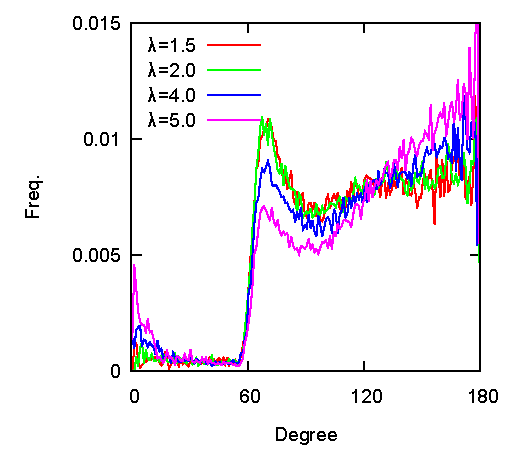
\includegraphics[width=\columnwidth]{./fig/Angle_Step.pdf}

\end{columns}

\begin{exampleblock}{ストランドの振る舞い}
\begin{itemize}
\item
ボンド長は伸びないが、アングルが増加。
\item
クーン・セグメント数は増加。
\end{itemize}
\end{exampleblock}


\end{frame}





%%%%%%%%%%%%%%%%%%%
\section{おわりに}
%%%%%%%%%%%%%%%%%%%

%%%%%%
\begin{frame}
\frametitle{おわりに}

\begin{exampleblock}{本研究の目標とアプローチ}
\begin{itemize}
\item
目標\\
破壊耐性に優れた軽量材料の創成とその設計指針の明確化
\item
アプローチ
	\begin{itemize}
	\item
	可逆性に優れた材料としてゴム材料を選択。
	\item
	構造明確なネットワークの構築のために超分子ネットワーク。
	\item
	既知のモデルとの整合性を確認。
	\item
	\color{red}シミュレーションの併用でマルチスケールモデルを構築\color{black}
	\end{itemize}
\end{itemize}
\end{exampleblock}


\begin{block}{KG 鎖のネットワークのMDシミュレーション}
KG 鎖によるネットワークのMDシミュレーションを行い、
\begin{itemize}
\item
KG 鎖によるネットワークにより、メゾスケールと構成方程式はつながる。
\item
KG 鎖の特徴を考慮すれば、ミクロなふるまいも検討可能
\end{itemize}
\end{block}

\end{frame}


%%%%%%%%%%%%%%%%%%%%%%%%%%%%%%%%%%%%%%%%%%%%%%%%%%%%%%%%%%%%%%%%%%%%%%%%%%%%%%%%%%%%%%%%%%
\begin{appendix}
%%%%%%%%%%%%%%%%%
\begin{frame}
\LARGE{補足資料}
\end{frame}
%%%%%%%%%%%%%%%%


%%%%%%%%%%%%%%%%%%%%%%%%%%
\section{KG鎖}
\subsection{KG鎖}
%%%%%%%%%%%%%%%%%%%%%%%%%%%%
\begin{frame}
\frametitle{KG鎖の平衡シミュレーションの条件}

長さの異なるKG鎖の平衡シミュレーションの条件

\begin{itemize}
\item
初期緩和:\\$\tau_{E2E}$ の 20 倍程度
\item
本計算:\\$0.1 \times \tau_{E2E} \times$ 800 ステップ
\end{itemize}

それぞれの長さの場合の計算条件を示した。

\begin{table}[htb]
\begin{center}
{
\begin{tabular}{c c c c c} \hline
Seg.	& 本数	& $\tau_{E2E}$	& Init. Relux.($\tau$)	& Main ($\tau$)	\\ \hline \hline	
10		& 200	& 1.0E2			& 1.0E4				&	1.0E1 $\times$ 800 steps \\ \hline	
20		& 200	& 4.1E2			& 5.0E4				&	5.0E2 $\times$ 800 steps \\ \hline	
30		& 200	& 1.1E3			& 1.0E5				&	1.0E2 $\times$ 800 steps \\ \hline	
40		& 200	& 1.9E3			& 2.0E5				&	2.0E2 $\times$ 800 steps \\ \hline	
50		& 200	& 3.6E3			& 4.0E5				&	4.0E2 $\times$ 800 steps \\ \hline
\end{tabular}
}
\end{center}
\end{table}

\end{frame}


%%%%%%%%%%%%%%%%%
\begin{frame}
\frametitle{平衡シミュレーションの結果}

長さの異なるKG鎖の平衡シミュレーションの結果を以下に示した。

\begin{table}[htb]
 \centering
 \begin{tabular}{c c c c c} \hline
Seg.	& Bonds	& Ave. Bond Len.	& $\langle R^2 \rangle$	& $C_{N}$	\\ \hline \hline	
10		& 9		& 0.965				& 13.0			& 1.55			\\ \hline	
20		& 19	& 0.965				& 29.3			& 1.65			\\ \hline	
30		& 29	& 0.965				& 46.2			& 1.71			\\ \hline	
40		& 39	& 0.965				& 63.7			& 1.75			\\ \hline	
40		& 49	& 0.965				& 79.9			& 1.75			\\ \hline
 \end{tabular}
\end{table}

\vspace{-5mm}
\begin{align*}
C_{\infty} = \dfrac{\langle R^2 \rangle}{N b^2}
\end{align*}
\end{frame}

%%%%%%
\begin{frame}
%[shrink squeeze]
%[allowframebreaks]
\frametitle{KG 鎖のポテンシャル}

\small
非結合ポテンシャル:ビーズ間に LJ ポテンシャル $U_{LJ}(r)$
\begin{align*}
U_{LJ}(r) &= 
\begin{cases}
4 \epsilon\left[\left(\dfrac{\sigma}{r}\right)^{12} - \left(\dfrac{\sigma}{r}\right)^{6} + \dfrac{1}{4} \right] \;\;\; & r< 2^{1/6} \sigma \\[8pt]
0 \;\;\; & r \geq 2^{1/6} \sigma
\end{cases}
\end{align*}

ボンドポテンシャル:FENE-LJ ポテンシャル $U_{FENE}$
\begin{align*}
U_{FENE}(r) &= 
\begin{cases}
-\dfrac{K}{2}\dfrac{\epsilon R_0^2}{\sigma^2} \ln \left[1-\left(\dfrac{r}{R_0}\right)^2 \right] \;\;\; & if \; r< R_0 \\[8pt]
\infty \;\;\; & otherwise
\end{cases}
\end{align*}

なお、一般的なパラメタセットは、
\begin{align*}
 \begin{cases}
	\epsilon = \sigma = 1 \\
	R_0 = 1.5 \\
	K=30
 \end{cases}
\end{align*}
\end{frame}

%%%%%%%%%%%%%%%%%%%%%%%%%
\subsection{各種特性}
%%%%%%%%%%%%%%
\begin{frame}
\frametitle{KG鎖のアングル}

\begin{columns}[totalwidth=1\textwidth]
\column{.5\textwidth}
\footnotesize
\begin{itemize}
\item
生データをヤコビアンで処理したものと合わせて示した。
\item
ビーズ間の 1,3 位の反発により、アングルが規制されていた。
\item
単純に算術平均した場合の値を図中に示した。
\end{itemize}


\column{.5\textwidth}
\begin{figure}
\centering
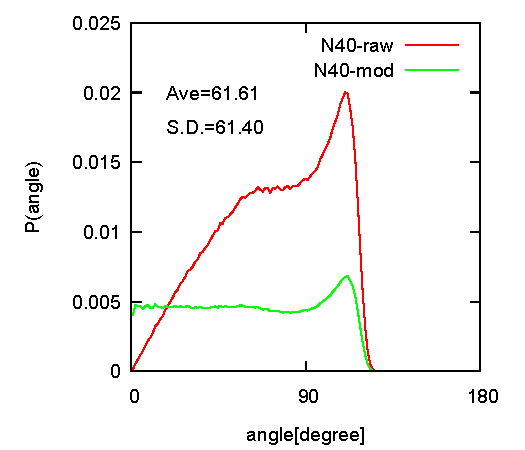
\includegraphics[width=60mm]{./fig/Angle_N40.pdf}
\end{figure}
\end{columns}

\end{frame}


%%%%%%%%%%%%%%%%%%
\begin{frame}
\frametitle{KG 鎖の特性比}

\footnotesize
1,3 位の反発をポテンシャルに基づき考慮すると、アングルの平均値は以下のように見積もれる。

\begin{align*}
&\langle \cos (\theta) \rangle 
= \dfrac{
\displaystyle \int_0^{\pi} \rm{d} \theta 
\sin(\theta) 
\color{red}
\cos(\theta)
\color{black} 
\exp \left(-\dfrac{U_{LJ}(r(\theta))}{k_B T}\right)
}
{\displaystyle \int_0^{\pi} \rm{d} \theta 
\sin(\theta) \exp \left(-\dfrac{U_{LJ}(r(\theta))}{k_B T}\right)}
\simeq 0.274 \notag \\
&\theta \simeq 74.1
\end{align*}

%ただし、
%\begin{align*}
%r(\theta)&=2b \sin \left( \dfrac{\pi-\theta}{2} \right) \notag \\[12pt]
%U_{LJ}(r) &= 
%\begin{cases}
%4 \epsilon\left[\left(\dfrac{\sigma}{r}\right)^{12} - \left(\dfrac{\sigma}{r}\right)^{6} + \dfrac{1}{4} \right] \;\;\; & r< 2^{1/6} \sigma \\[8pt]
%0 \;\;\; & r \geq 2^{1/6} \sigma
%\end{cases}
%\end{align*}

したがって、
\begin{align*}
\langle R^2 \rangle
&= (N-1) b^2
\left( 
\dfrac{1+ \langle \cos (\theta) \rangle}{1 - \langle \cos (\theta) \rangle}
-\dfrac{1}{N-1}
\dfrac{2 \langle \cos (\theta) \rangle(1-\langle \cos (\theta) \rangle^{N-1})}
{(1-\langle \cos (\theta) \rangle)^2}
\right) \\
\therefore 
C_{N} &= 
\left( 
\dfrac{1+ \langle \cos (\theta) \rangle}{1 - \langle \cos (\theta) \rangle}
-\dfrac{1}{N-1}
\dfrac{2 \langle \cos (\theta) \rangle(1-\langle \cos (\theta) \rangle^{N-1})}
{(1-\langle \cos (\theta) \rangle)^2}
\right)
\end{align*}
\end{frame}

%%%%%%%%%%%%%%%%%%
\begin{frame}
\frametitle{KG 鎖の特性比}

\begin{columns}[totalwidth=1\textwidth]
\column{.5\textwidth}
\footnotesize
長さの異なるKG鎖の平衡シミュレーションの結果を以下に示した。

\begin{table}[htb]
 \centering
 \begin{tabular}{c c c c c} \hline
Seg.	& Bond Len.	& $\langle R^2 \rangle$	& $C_{N}$	\\ \hline \hline	
10		& 0.965		& 13.0			& 1.55			\\ \hline	
20		& 0.965		& 29.3			& 1.65			\\ \hline	
30		& 0.965		& 46.2			& 1.71			\\ \hline	
40		& 0.965		& 63.7			& 1.75			\\ \hline	
40		& 0.965		& 79.9			& 1.75			\\ \hline
 \end{tabular}
\end{table}

\vspace{-5mm}
\begin{align*}
C_{N} = \dfrac{\langle R^2 \rangle}{N b^2}
\end{align*}

J.C.P.の論文記載のデータも併せて示した。

\column{.5\textwidth}
\begin{figure}
\centering
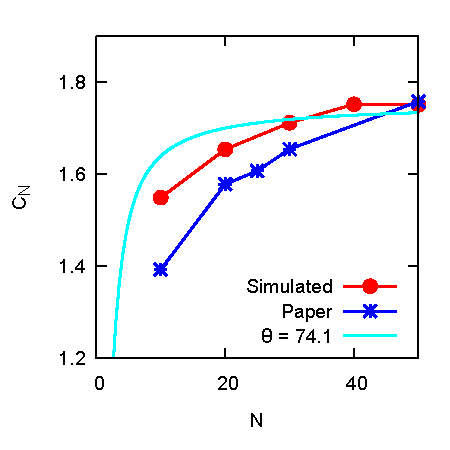
\includegraphics[width=60mm]{./fig/C_ratio.pdf}
\end{figure}
\end{columns}
\end{frame}

%%%%%
\begin{frame}
\frametitle{ボンドポテンシャル}

\begin{columns}[totalwidth=1\textwidth]

\scriptsize
\column{.5\textwidth}

KG 鎖においてのボンドポテンシャルは、LJ ポテンシャル $U_{LJ}$ と伸びきりバネの FENE ポテンシャル $U_{FENE}$ との和である $U_{FENE-LJ}(r)$ を用いている。
\begin{align*}
U_{FENE-LJ}(r) &= 
U_{LJ} + U_{FENE}
\end{align*}

これを、伸びきりの無い線形バネポテンシャル $U_{Harm}$ と組み合わせることもできる。
\begin{align*}
U_{Harm} = \dfrac{K}{2}(r-r_0)^2 
\end{align*}

$K=100, R_0=1.0$ のポテンシャルも併せて示した。
\column{.5\textwidth}
\begin{figure}
\centering
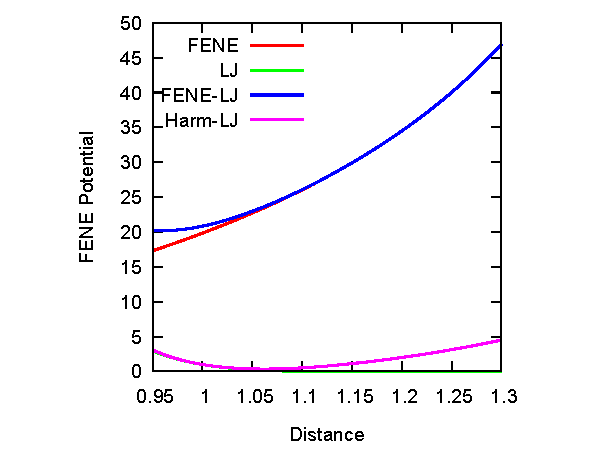
\includegraphics[width=60mm]{./fig/FENE.pdf}
\end{figure}
\end{columns}
\end{frame}

%%%%%%%%%%%
\begin{frame}
\frametitle{鎖の交差}
\footnotesize
$U_{FENE-LJ}(r)$ の二つのポテンシャルを設定することにより、KG 鎖においては鎖同士のすり抜けを抑制している。
この抑制効果を、上述のポテンシャルからエネルギー的に確認しよう。

\scriptsize
\begin{columns}[totalwidth=1\textwidth]
\column{.5\textwidth}
二本のポリマー鎖が、任意のボンドが直交するように接近した場合を考える。

エネルギーバリアーが最大となる場合は、ボンドが直角に重なった場合と考えられるので、この時のボンド長を $l$ とすると、異なる鎖に属するビーズ間の距離は、$\dfrac{\sqrt{2}}{2}l$ となる。ボンドは二本あり、非結合相互作用は四個あるので、一本の鎖当たりでは、
\tiny
\begin{align*}
U_{cross}
	&=U_{FENE}(r=l) +  2\times U_{LJ}(r=\dfrac{\sqrt{2}}{2}l)
\end{align*}

\column{.5\textwidth}
\begin{figure}
\centering
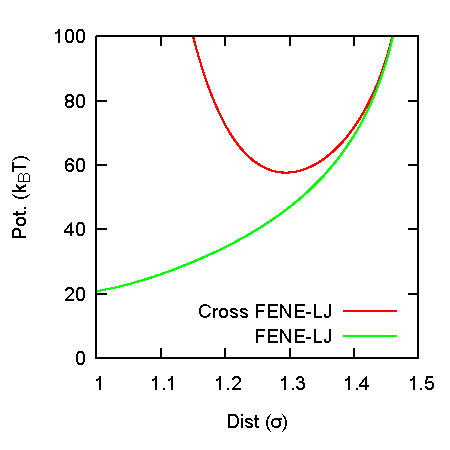
\includegraphics[width=50mm]{./fig/Cross_KG.pdf}
\end{figure}
\end{columns}

したがって、鎖の交差に対するポテンシャルは、約 $60 k_BT$ 程度と見積もれた。
\end{frame}

%%%%%%%%%%%%%%%%%%%%%%%%%%%%%%%%%%%%%%%%
\begin{frame}
\frametitle{アングルポテンシャルの導入}

\begin{columns}[totalwidth=1\textwidth]
\column{.5\textwidth}
非結合ポテンシャルを切って、$U_{FENE-LJ}$ のみを働かせると、自由連結鎖としての振る舞いを示すことは、すでに確認している。

ここに、アングルポテンシャルを入れてみる。
\column{.5\textwidth}
\begin{figure}
\centering
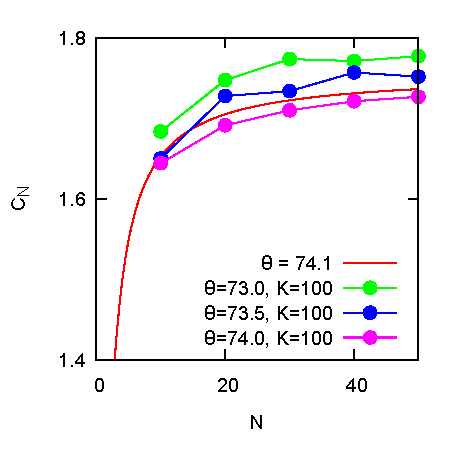
\includegraphics[width=60mm]{./fig/C_ratio_angle.pdf}
\end{figure}
\end{columns}

\end{frame}

%%%%%%%%%%%%%%%%%%%%%%%%%%%%%%%%%%%
\begin{frame}
\frametitle{ボンドポテンシャルの変更}

ボンドポテンシャルとして、線形バネを用いることを考える。

\scriptsize
\begin{columns}[totalwidth=1\textwidth]
\column{.5\textwidth}
二本のポリマー鎖が、任意のボンドが直交するように接近した場合を考える。

エネルギーバリアーが最大となる場合は、ボンドが直角に重なった場合と考えられるので、この時のボンド長を $l$ とすると、異なる鎖に属するビーズ間の距離は、$\dfrac{\sqrt{2}}{2}l$ となる。ボンドは二本あり、非結合相互作用は四個あるので、一本の鎖当たりでは、
\tiny
\begin{align*}
U_{cross}
	&=U_{Harm}(r=l) +  2\times U_{LJ}(r=\dfrac{\sqrt{2}}{2}l)
\end{align*}

このとき、
\begin{align*}
U_{Harm} = \dfrac{K}{2}(r-r_0)^2 
\end{align*}

\column{.5\textwidth}
\begin{figure}
\centering
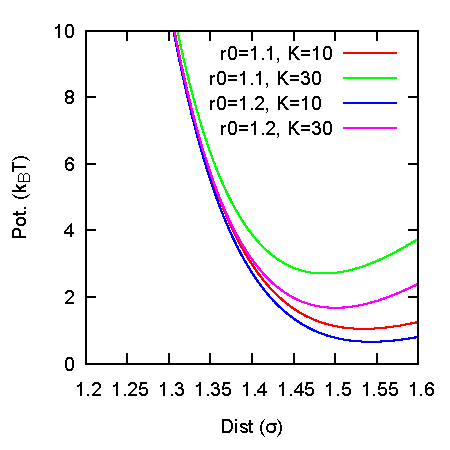
\includegraphics[width=50mm]{./fig/Cross_Harm_LJ.pdf}
\end{figure}
\end{columns}

\end{frame}

%%%%%%%%%%%%%%%%%%%%%%%%%%%%%%%%%%%%%%
\section{ファントムネットワークの理論}
%%%%%%%%%%%%%%%%%%%%%%%%%%%%%%%%%%%%%%
%%%%%%%%%%%%%%%%%%%%%%%%%%%%%%%%%%%%%%%%%%%%%%
\subsection{ファントムネットワークの振る舞い}
%%%%%%%%%%%%%%%%%%%%%%%%%%%%%%%%%%%%%%%%%%%%%%
%%%%%%%%%%%%%%
\begin{frame}
\frametitle{ファントムネットワークのゆらぎ}

\begin{columns}[totalwidth=1\textwidth]
\column{.47\textwidth}
\scriptsize
\begin{block}{ゆらぎの入ったポテンシャル}
ストランドの末端間ベクトル $\bm{R}_{nm}$ を、\\架橋点の位置ベクトル $\bm{r}_n$ を用いて、
\vspace{-3mm}
\begin{equation*}
\bm{R}_{nm} \equiv \bm{r}_n-\bm{r}_m
\end{equation*}

系のポテンシャルエネルギーは、
\vspace{-3mm}
\begin{equation*}
U=\dfrac{k}{2} \sum_{\langle nm \rangle} \bm{R}_{nm}^2
\end{equation*}

これは、自然長で決まる定数項と、ゆらぎに起因した第二項に分割でき、その和で以下となる。
\vspace{-3mm}
\begin{equation*}
U=\dfrac{k}{2} \sum_{\langle nm \rangle} {\bm{R}_{nm}^{(0)}}^2 + \dfrac{k}{2} \sum_{\langle nm \rangle} \Delta \bm{R}_{nm}^2
\end{equation*}
\end{block}

\column{.47\textwidth}
\scriptsize
\begin{block}{アンサンブル平均の二つの表式}
\vspace{-5mm}
\begin{align*}
 \begin{cases}
	\langle U \rangle = N_{strands} \dfrac{k}{2} \langle \Delta \bm{R}^2 \rangle \\
	\langle U \rangle = 3(N_{nodes}-1) \dfrac{1}{2} k_B T
 \end{cases}
\end{align*}
なお、第二式は等分配側より導出した。
\end{block}

\begin{exampleblock}{ファントムネットワークでのゆらぎ}
架橋点数 $N_{nodes}$、架橋点官能基数 $f$ とすれば、規則格子での一般式として、
\vspace{-3mm}
\begin{equation*}
\langle \Delta \bm{R}^2 \rangle = \dfrac{3k_B T}{k} \dfrac{2}{f} \left( 1-\dfrac{1}{N_{nodes}} \right)
\end{equation*}

適切な条件で、ストランドの自然長 $R_0$\\
を用いて、
\vspace{-3mm}
\begin{equation*}
\color{red}
\langle \Delta \bm{R}^2 \rangle = \dfrac{2}{f} R_0^2
\end{equation*}
\vspace{-6mm}
\end{exampleblock}

\end{columns}

\end{frame}


%%%%%%%%%%%%%%%%%
\begin{frame}
\frametitle{ファントムネットワークの振る舞い}

\begin{columns}[totalwidth=1\textwidth]
\column{.47\textwidth}
\scriptsize
\begin{block}{ストランドの末端間距離}
ストランドの末端間距離の分布関数は、畳み込み積分の形で、
\vspace{-3mm}
\begin{equation*}
\Omega(\bm{R}) = \Phi(\bar{\bm{R}}) + \Psi(\bm{\Delta R})
\end{equation*}

ダイヤモンド構造でのストランド末端間距離の $x$ 成分の分布関数 $P_{strand}(x)$ は、\vspace{-3mm}
\begin{align*}
P_{strand}(x) 
&= \dfrac{1}{2}\dfrac{1}{\sqrt{2\pi}\Delta_{\lambda}^x} \\
&\times \left[ \exp\left(-\dfrac{(x-X_{\lambda})^2}{2(\Delta_{\lambda}^x)^2} \right) \right. \\
&\quad \left. + \exp\left(-\dfrac{(x+X_{\lambda})^2}{2(\Delta_{\lambda}^x)^2} \right) \right]
\end{align*}
なお、$X_{\lambda}$、$\Delta_{\lambda}^x$ は、伸長比 $\lambda$ である時の、ストランド長及びゆらぎの $x$ 成分を表す。
\end{block}

\column{.47\textwidth}
\scriptsize
\begin{block}{ずり弾性率 $G_{ph}$}
ファントムネットワークでのずり弾性率 $G_{ph}$ は、以下の表式で表される。
\vspace{-3mm}
\begin{align*}
G_{ph} &= \dfrac{1}{3} \dfrac{1}{V} \left. \dfrac{d^2 F_{ph}}{d \lambda^2} \right|_{\lambda = 1}\\
&=\dfrac{\langle R_{strand}^2 \rangle}{\langle R_0^2 \rangle} \nu k_B T
\end{align*}
ここで、$\nu$ は、ストランドの数密度である。

\vspace{3mm}
ダイヤモンド構造のように規則構造からなるネットワークにおいて、各ストランド長がガウス鎖の二乗平均末端距離となるようにシステムサイズを設定した場合、$\langle R_{strand}^2 \rangle = \langle R_0^2 \rangle$ であるので、
\vspace{-3mm}
\begin{align*}
\color{red}
G_{ph}= \nu k_B T
\end{align*}

\end{block}
\end{columns}

\end{frame}




%%%%%%%%%%%%%%%%%%%%%%
\subsection{伸長時の振る舞い}
%%%%%%%%%%%%%%%%%
\begin{frame}
\frametitle{伸長時($\lambda =2$)の振る舞い}

\begin{columns}[T, totalwidth=0.96\linewidth]
\column{.47\linewidth}

伸長時 $\lambda =2$

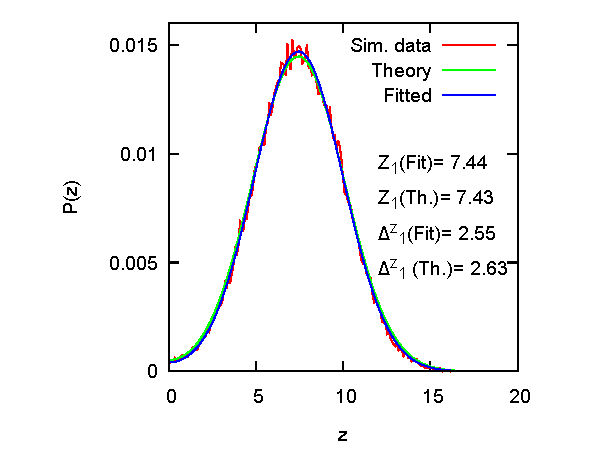
\includegraphics[width=55mm]{./fig/L2_Rz.pdf}

\column{.47\linewidth}
未伸長

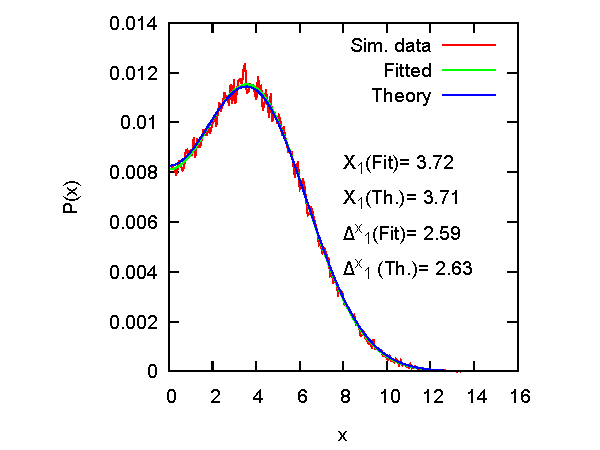
\includegraphics[width=55mm]{./fig/L1_Rx.pdf}
\end{columns}

\small
\begin{exampleblock}{未伸長との比較}
$z$ 軸方向に伸長した場合の一次元での末端間距離は、正確に二倍になった。

一方、ゆらぎは、理論的には不変なのであるが、5 \% 程度減少していた。
\end{exampleblock}

\end{frame}

\section{その他}


%%%%%%%%%%%%%%%%%
\begin{frame}
%[shrink squeeze]
\frametitle{高分子材料の疲労と破壊}

ガラス状態の高分子材料を考えた場合。

\begin{columns}[totalwidth=1\textwidth]
\column{.6\textwidth}
\begin{block}{破壊のモード(巨視的)}
脆性破壊 $\Leftrightarrow$ 延性破壊\\
脆性破壊は、降伏前にミクロなクラックが進展した破壊とも考えられる。
\end{block}
\column{.4\textwidth}
	\centering
	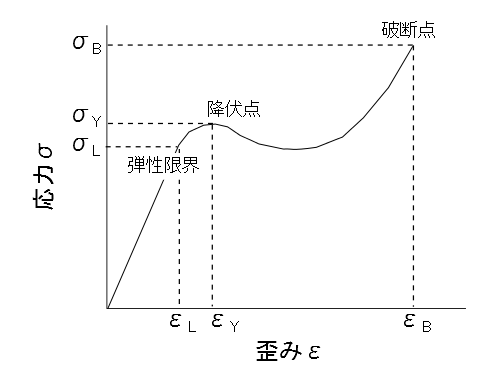
\includegraphics[width=35mm]{./fig/S_S_Curve.png}
\end{columns}


\begin{exampleblock}{降伏と劣化}
	\begin{itemize}
	\item
	靭性向上のため
	\begin{itemize}
		\item
		{\color{red} 局所的な降伏}が必須。(クレイズのような局所的な破壊も含む)
		\item 
		一般に、高分子材料の{\color{red} 降伏は不可逆}。
	\end{itemize}
	\item
	降伏による劣化
		\begin{itemize}
			\item 
			降伏 $\Leftrightarrow$ {\color{red} 本質的には、少しずつ破壊。}
			\item
			{\color{red} 破壊領域への水分の浸透 $\Leftarrow$ 長期耐久性の欠如}
		\end{itemize}
	\end{itemize}
\end{exampleblock}
\end{frame}


%%%%%%%%%%%%%%%%%%%
\begin{frame}
\frametitle{架橋点の近傍}

\centering
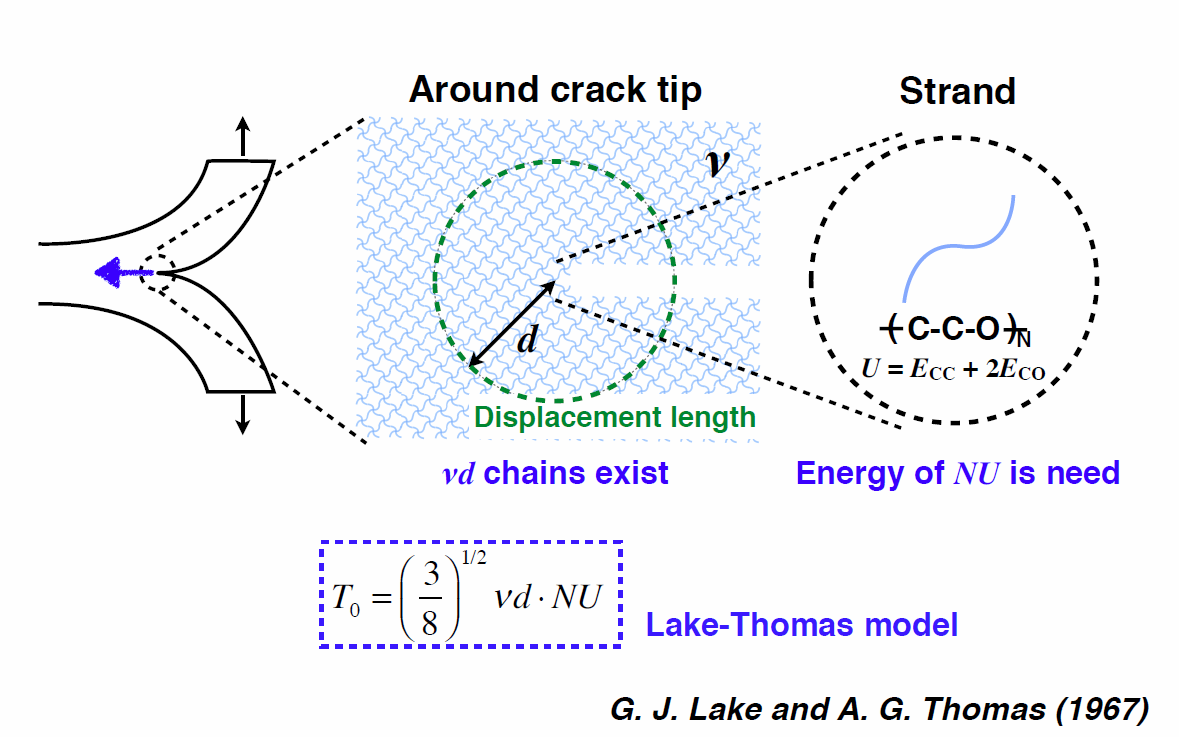
\includegraphics[width=80mm]{./fig/Lake_Thomas.png}

\end{frame}

%%%%%%%%%%%%%%%%%%%%%%%%%%%%%%%%%
\begin{frame}
%[shrink squeeze]
%[allowframebreaks]
\frametitle{ダイヤモンド構造のジオメトリ}

\begin{columns}[T, totalwidth=1\textwidth]
\column{.47\textwidth}
ダイヤモンド構造で、ストランド長 $r$、ユニットセル長さ $a$ とし、右下の緑の立方体に着目。

\begin{figure}
\centering
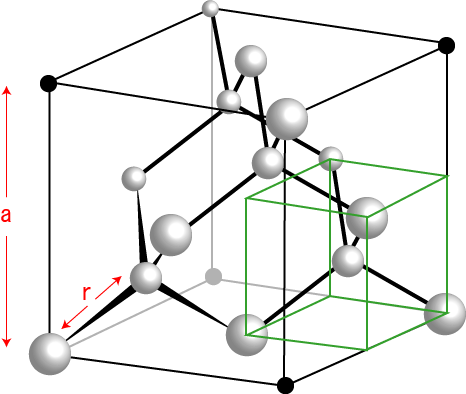
\includegraphics[width=40mm]{./fig/dia_green_2.png}
\end{figure}

\column{.47\textwidth}
この部分は、半径 $r$ の球に内接する正四面体であり、緑の立方体の対角線の長さは $2r$ となる。
\begin{figure}
\centering
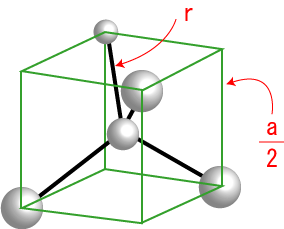
\includegraphics[width=40mm]{./fig/dia_mini_2.png}
\end{figure}
\end{columns}

\vspace{3mm}
\centering
したがって、三平方の定理を使って、
\vspace{-2mm}
\begin{align*}
\sqrt{3} \dfrac{a}{2} = 2r \Rightarrow {\color{red} a= \dfrac{4 r}{\sqrt{3}} }
\end{align*}
\end{frame}
%%%%%%%%%%%%%%%%%%%%%%%%%%%%%%%%%%%%%%%%%%%%%%%%
\begin{frame}
\frametitle{架橋点近傍の拘束状態に基づく二つのモデル}

\begin{columns}[totalwidth=1\textwidth]
\column{.5\textwidth}
ストランドと架橋点の模式図
%\centering
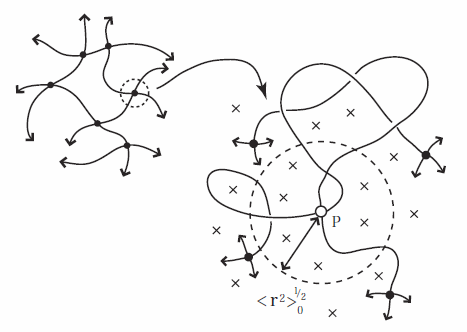
\includegraphics[width=55mm]{./fig/JP_vicinity.png}

架橋点はストランド経由で直接連結した架橋点(図中の黒丸)以外の、近接する多数のストランド及び架橋点(図中の×)に囲まれている。

\column{.5\textwidth}
\begin{itemize}
\item
``Affine NW Model''\\
架橋点は周辺に強く拘束され巨視的変形と相似に移動。\\(Affine 変形)
\footnotesize
\begin{equation*}
G=\nu k_B T
\end{equation*}
\normalsize
$\nu$ は、ストランドの数密度
\item
``Phantom NW Model''\\
架橋点が大きく揺らぎ、実効的なずり弾性率($G$)が低下。
\footnotesize
\begin{align*}
G&=\xi \nu k_B T \\
\xi&= 1 -\dfrac{2}{f}
\end{align*}
\normalsize
$f$ は架橋点の分岐数
\end{itemize}
\end{columns}

\end{frame}

%%%%%%%%%%%%%%%%
\begin{frame}
\frametitle{伸び切り鎖のモデル}

図から明らかなように、``3-Chain model'' は、一軸伸長において、伸長方向への伸びきり効果を過剰評価している。

積分の形とした ''Full-Chain model'' においても、その効果は大きいようである。

しかしながら、''8-Chain model'' の過小評価が妥当かどうかもはっきりしない。

\centering
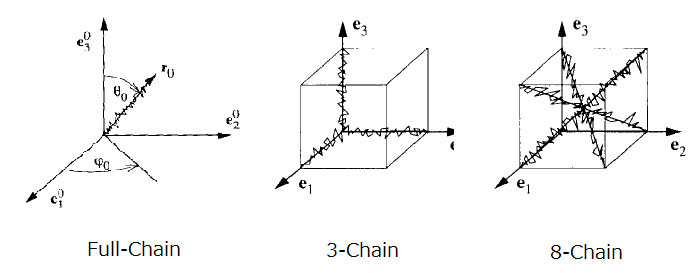
\includegraphics[width=100mm]{./fig/Stretched_Chain.png}

\end{frame}



\begin{frame}
\frametitle{MD シミュレーションの応力}

\begin{align*}
\overleftrightarrow{\sigma} V
&=\sum_i m_i \bm{v}_i \bigotimes m_i \bm{v}_i \\
&+\sum_{(i<j)} \dfrac{\bm{r}_{ij} \bigotimes \bm{r}_{ij}}{\bm{r}_{ij}}
\left( \dfrac{\diff U_{FENE}(\bm{r})}{\diff \bm{r}} \right)_{r=r_{ij}} \\
&+\sum{(i<j)} \dfrac{\bm{r}_{ij} \bigotimes \bm{r}_{ij}}{\bm{r}_{ij}}
\left( \dfrac{\diff U_{LJ}(\bm{r})}{\diff \bm{r}} \right)_{r=r_{ij}}
\end{align*}

\end{frame}



%%%%%%%%%%%%%
\begin{frame}
\frametitle{伸長速度の比較}

\begin{columns}[totalwidth=1\textwidth]
\column{.5\textwidth}
\tiny
\begin{align*}
\overleftrightarrow{\sigma} V
&=\sum_i m_i \bm{v}_i \bigotimes m_i \bm{v}_i \\
&+\sum_{(i<j)} \dfrac{\bm{r}_{ij} \bigotimes \bm{r}_{ij}}{\bm{r}_{ij}}
\left( \dfrac{\diff U_{FENE}(\bm{r})}{\diff \bm{r}} \right)_{r=r_{ij}} \\
&+\sum{(i<j)} \dfrac{\bm{r}_{ij} \bigotimes \bm{r}_{ij}}{\bm{r}_{ij}}
\left( \dfrac{\diff U_{LJ}(\bm{r})}{\diff \bm{r}} \right)_{r=r_{ij}}
\end{align*}

\column{.5\textwidth}
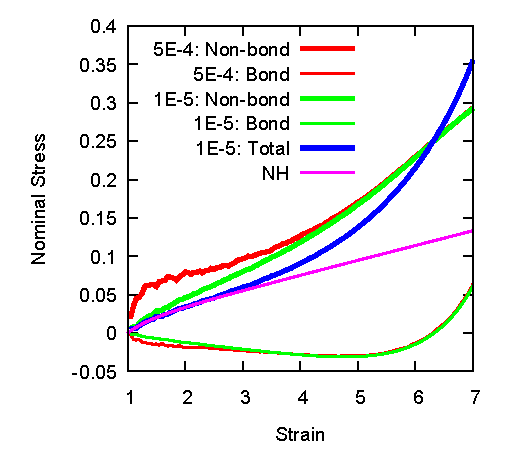
\includegraphics[width=\columnwidth]{./fig/SS_bond.pdf}
\end{columns}

\begin{block}{KG 鎖の振る舞い}
\begin{itemize}
\item
伸長速度 $\sigma/\tau = 5E^{-4}$ [$\sigma/\tau$] では、ノンボンドの寄与が大きく増加
\item
セグメント間での相互作用が応力の増加に寄与。
\end{itemize}
\end{block}

\end{frame}


\end{appendix}

\end{document}
